\section{UC2: Planlæg åbning}

\subsection{Linux Platform / DevKit8000}

Enkelte extensions er udeladt på sekvensdiagrammet, da de blot resulterer i en terminering af use-case-sekvensen.

\begin{figure}[H]
	\caption{Klassediagram UC2: Planlæg åbning på DevKit8000}
	\label{CD:UC2-devkit}
	\includegraphics[scale=0.35]{CD-planlaeg-åbning-Linux-platform}
\end{figure}

\begin{figure}[H]
	\caption{Sekvensdiagram UC2: Planlæg åbning på DevKit8000}
	\label{SD:UC2-devkit}
	\includegraphics[scale=0.4]{SD-planlaeg-åbning-Linux-platform}
\end{figure}

\subsection{PSoC 5}
\begin{figure}[H]
	\caption{Klassediagram UC2: Planlæg åbning på PSoC 5}
	\label{CD:PSoC:UC2-1}
	\includegraphics[scale=0.35,trim=0 0 0 0, clip]{APPSoC/UC2-CD-planlaeg-aabning-PSoC}
\end{figure}

\begin{figure}[H]
	\caption{Sekvensdiagram UC2: Planlæg åbning på PSoC 5}
	\label{SD:PSoC:UC2}
	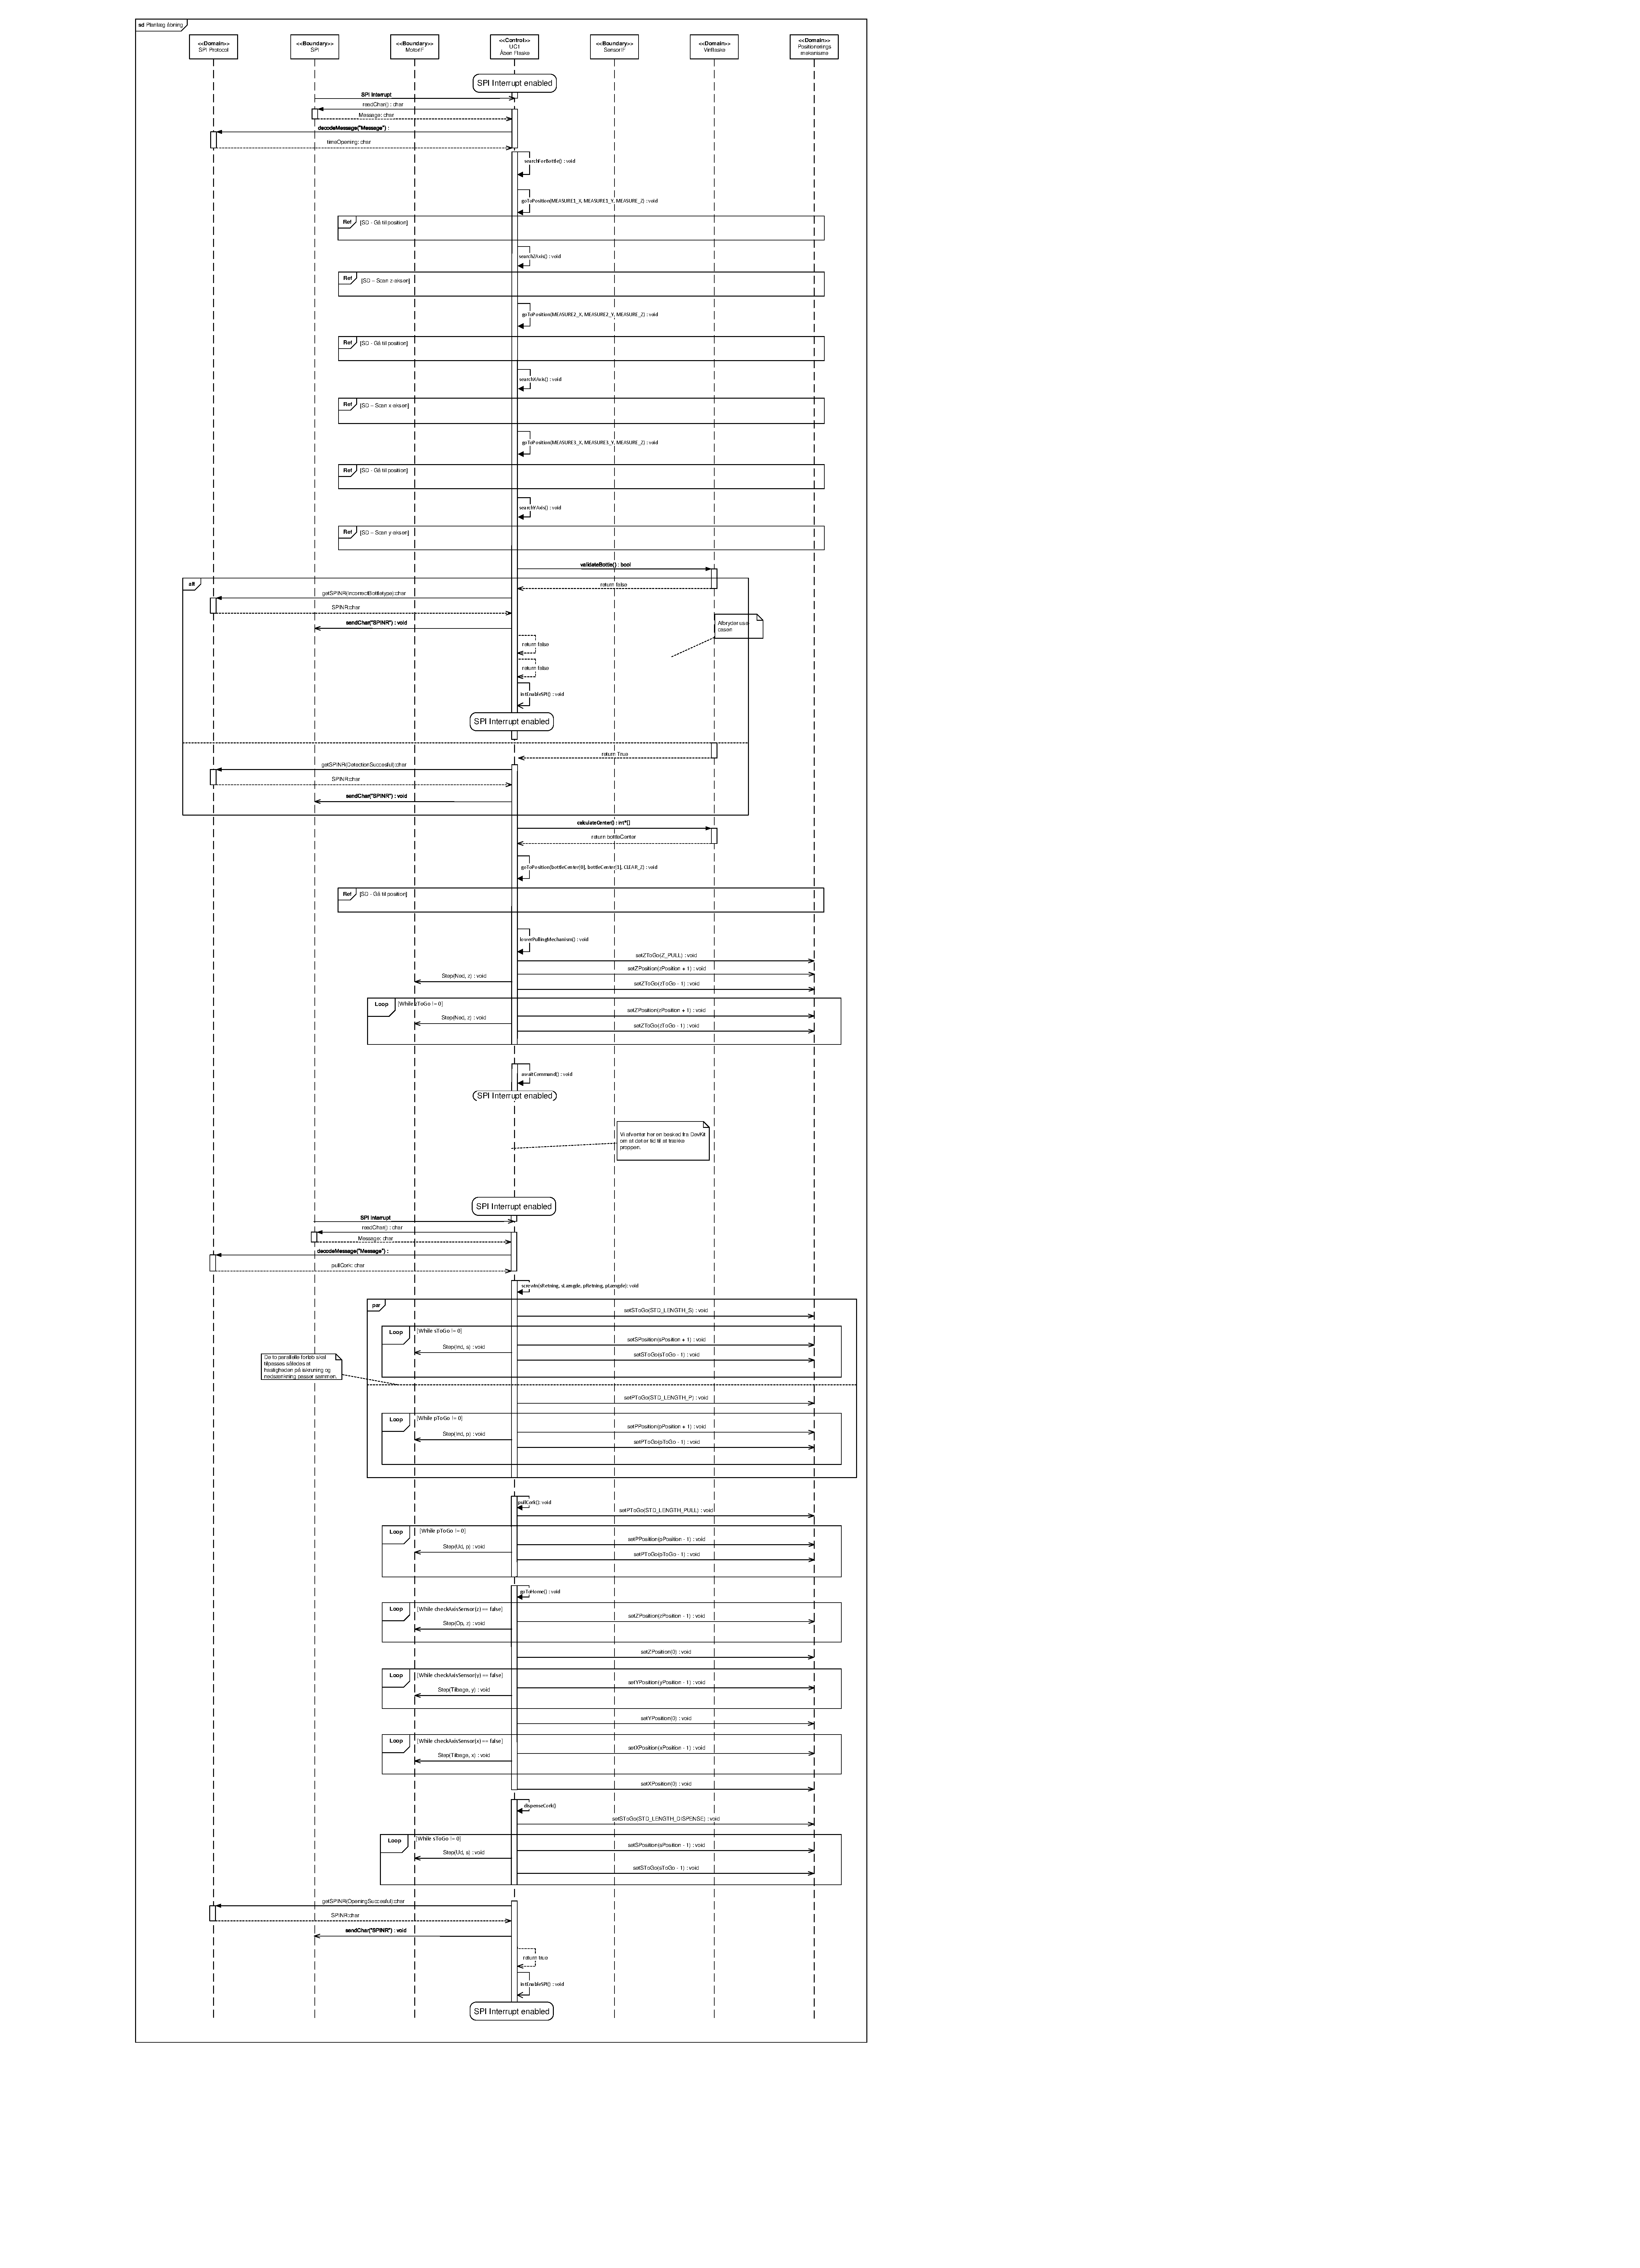
\includegraphics[scale=0.18,trim=0 0 0 0, clip]{APPSoC/UC2-planlaeg-aabning-v1-simplified}
\end{figure}